\documentclass[a4paper,12pt]{article}
\usepackage[T1]{fontenc}
\usepackage{ninecolors}
\usepackage{booktabs}
\usepackage{caption}
\usepackage{tabularray}
\usepackage{hyperref}
\usepackage{graphicx}
\usepackage{subcaption}
\usepackage{parskip}
\usepackage{tikz}
\usepackage{circuitikz}
\usepackage[tocentry]{vhistory}
\usepackage{float}
\hypersetup{
  colorlinks=true,
  linkcolor=blue,
  filecolor=magenta,
  urlcolor=cyan,
  pdftitle={Fur Face},
  pdfpagemode=FullScreen,
}
\graphicspath{ {img/} }
\captionsetup[table]{position=bottom}
\usepackage{geometry}
\usepackage{siunitx}
\usepackage{awesomebox}

\tikzset{
  padStyle/.style={line width=1mm, draw=orange, fill=none}
}

\tikzset{
  partStyle/.style={line width=1mm, draw=black, fill=none, rounded corners=4pt}
}

\begin{document}

\begin{titlepage}
  \vspace*{\stretch{1.0}}
  \begin{center}
    \Large\textbf{Fur Face}\\
    \large{Effect Pedal Kit by Pedal Markt}
  \end{center}
  \vspace*{\fill}
  \begin{center}
    \today
  \end{center}
\end{titlepage}

\tableofcontents
\pagebreak

\section{Introduction}

Fur Face is our take on a classic fuzz circuit. It sounds
great on string instruments, guitars, synths and drum
machines. It's a hefty, in your face silicon fuzz.

Enclosures for Fur Face and other pedals in the Beastly
Series were designed by \href{https://fiz.gallery/}{Agata
Fiz.}

\begin{figure}[h!]
  \centering
  \begin{subfigure}[b]{0.49\textwidth}
    \centering
    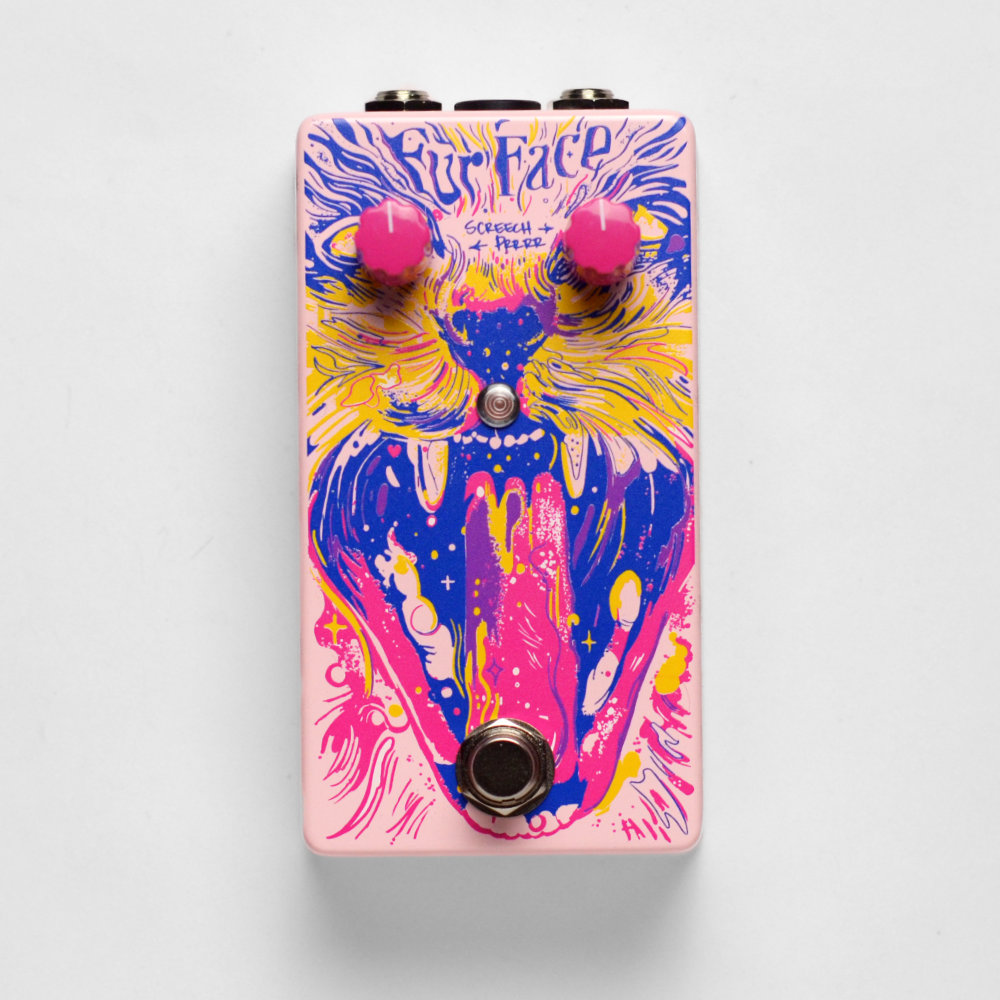
\includegraphics[width=\textwidth]{fur-face-front-1000.jpg}
  \end{subfigure}
  \begin{subfigure}[b]{0.49\textwidth}
    \centering
    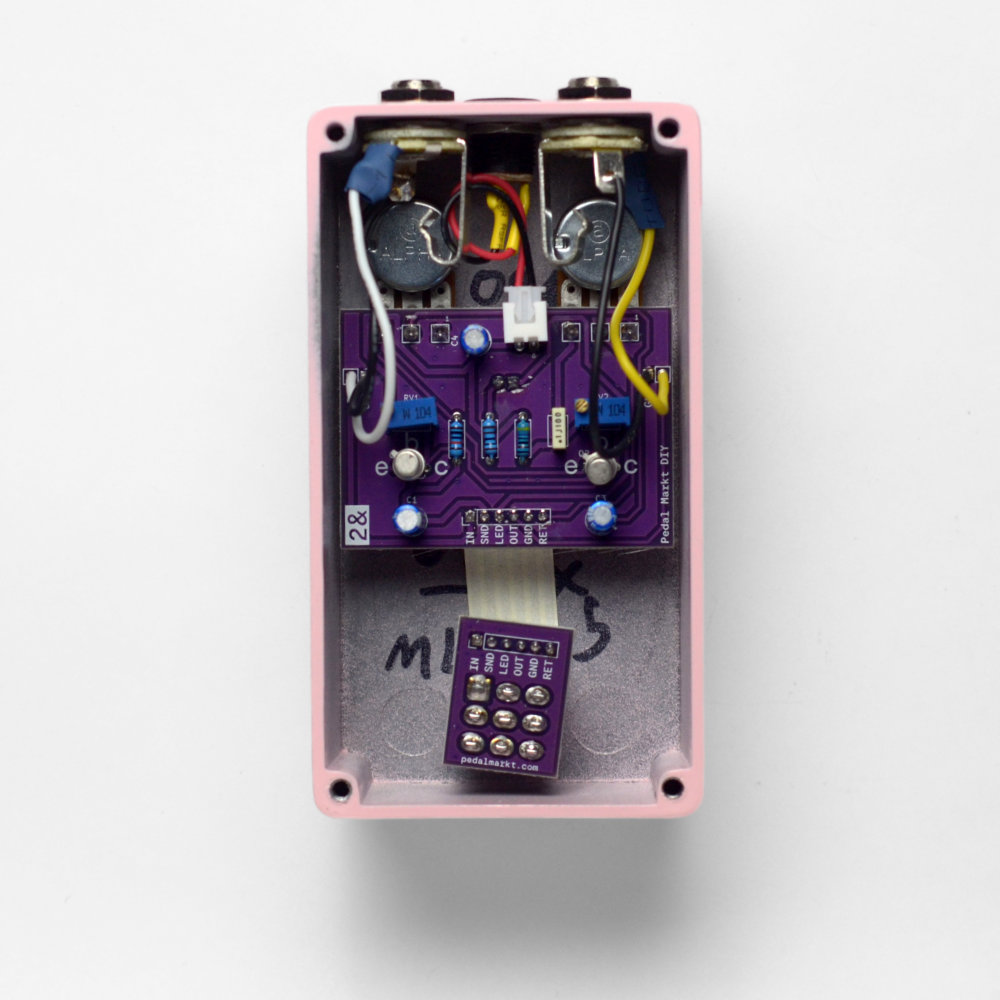
\includegraphics[width=\textwidth]{fur-face-inside-1000.jpg}
  \end{subfigure}
  \caption{Fur Face: oustide and inside}
  \label{fig:FurFace}
\end{figure}

Fur Face is designed to be easy to build and tune. The pedal
uses npn-transistors instead of traditional pnp to simplify
the power circuitry.

Fur Face has internal biasing pots for both transistors to
allow builders to experiment swapping parts and tuning the
device. We include recommended bias voltages for both
transistors. Feel free to use those as a starting point.
Part of the fun of this kit is exploring how bias affects
the sound of the pedal.

\pagebreak

\section{BOM – Bill of Materials}

BOM is a document that lists the parts you'd need to build a
project. Each row corresponds to a component with a certain
value, for example, a `ceramic capacitor with value 1nF.`
There could be one or more actual physical parts per
row, their designators are listed in the \textit{Reference}
column.

\tipbox{
  Components in the BOM are listed in order of assembly. Go
  through the table top to bottom. If you haven't built a
  kit before, check out the
  \hyperref[sec:steps]{Step-by-step Instructions} first.
}

\tipbox{
  In the BOM \textit{text in italic font} gives tips about how to mount or
  solder parts.
}

\tipbox{
  If you'd like to experiment with using different
  transistors, please socket them. See the guide
  \hyperref[sec:transistors]{here.}
}

\newgeometry{hmargin={1cm}}

\begin{longtblr}[caption = {BOM}]{
  hlines,
  vlines,
  rows={ht=1.2em},
  row{even}={bg=gray9},
  row{1}={bg=gray3,fg=white},
  width=\linewidth,
  colspec={llllX[2]},
}
  \hspace{1em}
  & \textbf{Ref}
  & \textbf{Value}
  & \textbf{Qnty}
  & \textbf{Description}
  \\
  \SetCell[c=5]{c,bg=gray6,fg=white}\textbf{Outboard}
  \\
  \hspace{1em}
  & – & Enclosure & 1 & \textit{Mount both pots, DC
  jack, Footswitch and Lampshade into the enclosure
  before soldering}
  \\
  \hspace{1em}
  & -- & Lampshade & 1
  & Small transparent plastic part for the LED,
  \textit{mount in enclosure before putting the boards in}
  \\
  \hspace{1em}
  & -- & Rubber Ring & 1
  & \textit{Use it to keep Lampshade in place}
  \\
  \hspace{1em}
  & -- & DC Jack & 1
  & Black plastic part with a nut, \textit{mount in
  enclosure before soldering}
  \\
  \hspace{1em}
  & -- & DC Cable & 1
  & Red and black cables in a JST connector, \textit{cut to
  $\approx5cm$ and solder to DC Jack once it's mounted in
  enclosure. Black wire to larger lug, red to the lug
  opposite it. Middle lug should stay unconnected.}
  \\
  \hspace{1em}
  & -- & Audio Jack & 2 & \textit{Only mount these in the
  enclosure together with the main board once they are wired up}
  \\
  \SetCell[c=5]{c,bg=gray6,fg=white}\textbf{Main board, floor side}
  \\
  \hspace{1em}
  & GND & Wire & 2 & $\approx8cm$, black, \textit{strip and
  tin the ends}
  \\
  \hspace{1em}
  & IN & Wire & 1 & $\approx8cm$, any color, \textit{strip and tin
  the ends}
  \\
  \hspace{1em}
  & OUT & Wire & 1 & $\approx8cm$, any other color,
  \textit{strip and tin the ends}
  \\
  \hspace{1em}
  & R2 & 1K & 1
  & Resistor for the LED, larger value will make the LED dimmer
  \\
  \hspace{1em}
  & R1 & 100K & 1 & Resistor
  \\
  \hspace{1em}
  & R3 & 470 & 1 & Resistor
  \\
  \hspace{1em} & Q1, Q2 & BC108 & 2 & Pinout:
  E=emitter, B=base, C=collector. \textit{See
  \hyperref[sec:transistors]{this section} if you'd like to
  try other transistors}
  \\
  \hspace{1em}
  & J1 & Power Socket & 1
  & JST 2-pin m, in the top-center part of the board
  \\
  \hspace{1em}
  & C2 & 100n & 1
  & Film capacitor
  \\
  \hspace{1em}
  & C1 & 2.2u & 1
  & Electrolytic capacitor, \textit{orientation matters}
  \\
  \hspace{1em}
  & C3 & 22u & 1
  & Electrolytic capacitor, \textit{orientation matters}
  \\
  \hspace{1em}
  & C4 & 47u & 1
  & Electrolytic capacitor, \textit{orientation matters}
  \\
  \hspace{1em}
  & RV1, RV2 & 100k & 2
  & Trimpots, \textit{orientation matters}
  \\
  \SetCell[c=5]{c,bg=gray6,fg=white}\textbf{Main board, player side}
  \\
  \hspace{1em}
  & -- & Ribbon cable & 1
  & Pads for that cable are in the bottom-center of the main
  board, \textit{solder one end to main board, another to
  switch board, \textbf{make sure pin names on the two
  boards match, IN on one board is connected to IN on the
  other board etc}}
  \\
  \hspace{1em}
  & RV3 (Screech) & B1k & 1
  & Potentiometer, \textit{mount in enclosure before
  soldering}
  \\
  \hspace{1em}
  & RV4 (Prrrr) & A500k & 1
  & Potentiometer, \textit{mount in enclosure before
  soldering}
  \\
  \hspace{1em}
  & -- & LED & 1
  & \textit{Insert in PCB first. Solder last, once the
  main board is in the enclosure. Orientation matters}
  \\
  \SetCell[c=5]{c,bg=gray6,fg=white}\textbf{Switch board, player side}
  \\
  \hspace{1em}
  & -- & Footswitch & 1
  & \textit{Mount in enclosure before putting the boards in}
  \\
\end{longtblr}

\restoregeometry{}

\subsection{Note on values}

Different kits and schematics designate values differently.
For example, these usually mean the same value:
\\
$\SI{2.2}{\kohm} = 2.2k = 2k2 = 2.2 \times 10^{3} Ohm = 2200Ohm$
\\
$\SI{4.7}{\uF} = 4.7u = 4u7 = 4.7 \times 10^{-6} Farad = 0.0000047 Farad$

\begin{table}[h!]
  \caption{Component values}
  \centerline{
    \begin{tblr}{
      hlines,
      vlines,
      rows={ht=1.2em},
      row{1}={bg=gray3,fg=white},
      colspec={Xrr}
    }
      \textbf{Value}
      & \textbf{Multiplier}
      & \textbf{Unit}
      \\
      \SetCell[c=3]{c}\textbf{Resistance}
      \\
      \SI{100}{\ohm}, 100R, 100 & 1 & Ohm
      \\
      \SI{1}{\kohm}, 1k & $10^{3}$ & Ohm
      \\
      \SI{1}{\Mohm}, 1M & $10^{6}$ & Ohm
      \\
      \SetCell[c=3]{c}\textbf{Capacitance}
      \\
      \SI{1}{\pF}, 1p & $10^{-12}$ & Farad
      \\
      \SI{1}{\nF}, 1n & $10^{-9}$ & Farad
      \\
      \SI{1}{\uF}, 1u & $10^{-6}$ & Farad
    \end{tblr}
  }
\end{table}

\pagebreak

\section{Experimenting with transistors}
\label{sec:transistors}

The circuit consists of just a handful of parts, and transistor
selection and bias play a huge role in the sound of the
pedal.

The stock transistors we use for Fur Face are BC108, Q1
biased to about \SI{1.3}{\V}, Q2 to about \SI{5.8}{\V}.

When inserting the transistors, please match their pinout to
the expected pinout indicated on the PCB: E to emitter, B to
base, C to Collector.

\begin{figure}[h!]
  \begin{center}
    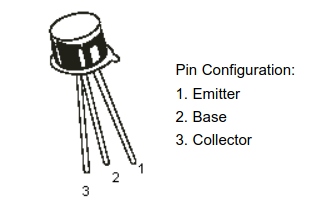
\includegraphics[width=0.7\textwidth]{bc108-pinout.png}
  \end{center}
  \caption{BC108 pinout}
\end{figure}


\section{Step-by-step Instructions}
\label{sec:steps}

\end{document}
